\chapter{Applications of Lagrange formalism}
In this chapter we will discuss some potential applications of the Lagrange picture of classical mechanics.
\section{Theory of small oscillations}
Many physical problems have an oscillatory nature but, when we try to solve those problems, we usually encounter difficult (sometimes impossible) differential equations.
For this reason we now introduce a systematic way to deal with oscillatory problems in the case of a small oscillation.
\subsection{$\mathbf{n = 1}$ degree of freedom systems}
Let's start with a 1 degree of freedom system. In this case the Lagrangian may look something like this:
\begin{equation}
    \lagr = \dfrac{1}{2}m\dot{q}^2 - V(q)
\end{equation}
Notice that we asked for a potential that only depends on the coordinate $q$.
We take in consideration the system near point of local minimum for the potential.
\begin{figure}[!ht]
    \centering
    \includesvg[width=0.6\textwidth]{res/svg/potential1Dapprox}
    \caption{1-D potential}
    \label{fig:image10}
\end{figure}
Given this we can approximate the potential to it's second order Taylor expansion near the point $q_0$ (local minimum):
\begin{equation}
    V \simeq V(q_0) + \cancel{\pdv{V}{q}\bigg|_{q_0}}(q-q_0) + \dfrac{1}{2}\pdv[2]{V}{q}\bigg|_{q_0}(q-q_0)^2
\end{equation}
The first derivative is zero since we are at a minimum, we can also ignore the value of the potential $V(q_0)$ and set it equal to zero, since we can always change the potential reference. Finally, we define:
\begin{equation}
    \eta \defineeq q-q_0
\end{equation}
And so we get:
\begin{equation} \label{e:potential_1D_oscillation}
    V(\eta) \simeq \dfrac{1}{2}\underbrace{\pdv[2]{V}{\eta}\bigg|_{q_0}}_{\Velegant}\eta^2 = \dfrac{1}{2}\Velegant\eta^2
\end{equation}
Where we defined the second order partial derivative as a known quantity $\Velegant$. We also know that, since $q$ and $\eta$ are different only for a constant term:
\begin{equation} \label{e:kinetic_1D_oscillation}
    T = \dfrac{1}{2}m\dot{q}^2 = \dfrac{1}{2}m\dot{\eta}^2
\end{equation}
From this we can write the \eleref :
\begin{equation}
    \begin{split}
        \dv{}{t}\pdv{\lagr}{\dot{\eta}} -\pdv{\lagr}{\eta} = 0 \\
        \dv{}{t}\pdv{T}{\dot{\eta}} + \pdv{V}{\eta} = 0
    \end{split}
\end{equation}
Substituting what we got in \eqref{e:potential_1D_oscillation} and \eqref{e:kinetic_1D_oscillation}:
\begin{equation}
    \begin{split}
        \dv{}{t}(m\dot{\eta}) + \Velegant\eta &= 0\\
        m\ddot{\eta} + \Velegant\eta &= 0
    \end{split}
\end{equation}
From which we get this condition:
\begin{equation} \label{e:condition_1D_oscillation}
    \ddot{\eta} =- \dfrac{\Velegant\eta}{m}
\end{equation}
We are searching for solutions of this type:
\begin{equation}
    \eta (t) = a\efunction^{-i\omega t}
\end{equation}
And so we evaluate the second order derivative:
\begin{eqnarray}
    \ddot{\eta} (t) = -a\omega^2\efunction^{-i\omega t}
\end{eqnarray}
We now impose the condition that $a\neq 0$ which is reasonable since $a=0$ would correspond to the absence of motion, so from \eqref{e:condition_1D_oscillation} we get:
\begin{equation}
    \begin{split}
        m\omega^2\cancel{a\efunction^{-i\omega t}} &= \Velegant\cancel{a\efunction^{-i\omega t}}\\
        \omega &= \pm \sqrt{\dfrac{\Velegant}{m}}
    \end{split}
\end{equation}
By convention we usually take the $+$ sign and refer to the other solution as $-\omega$. The general solution for $\eta$ will be of this form:
\begin{equation}
    \eta (t) = ca\efunction^{-i\omega t} + c'a\efunction^{i\omega t} = A \sin(\omega t + \varphi) = A \sin\brackets{\sqrt{\dfrac{\Velegant}{m}} t + \varphi}
\end{equation}
\subsection{$\mathbf{n\geq 2}$ degrees of freedom systems}
Now we want to discuss a more general type of system with $n\geq2$ degrees of freedom. Again we take in consideration a point $\vec{q}_0 = (q_{1,0}, q_{2,0},\dots,q_{n,0})$ of local minimum for the potential $V$ which now is a function of all the coordinates $q_{\alpha}$.
\begin{figure}[!ht]
    \centering
    \includesvg[width=0.6\textwidth]{res/svg/potential2Dapprox}
    \caption{2-D potential}
    \label{fig:image11}
\end{figure}
In this case the potential can be approximated near the point with the Taylor formula for multivariable scalar functions:
\begin{equation} \label{e:taylor_potential_scalar_product}
    V(\vec{q}) \simeq \underbrace{V(\vec{q}_0)}_{\text{constant}} + \\cancel{\langle \grad V(\vec{q}_0), \vec{q}-\vec{q}_0\rangle} + \dfrac{1}{2}\langle H V(\vec{q}_0)(\vec{q}-\vec{q}_0), (\vec{q}-\vec{q}_0)\rangle
\end{equation}
Again we exploit the fact that we can choose an arbitrary level for the potential, and we define:
\begin{equation}
    \eta_{\alpha} = q_{\alpha} - q_{\alpha,0}
\end{equation}
Expanding \eqref{e:taylor_potential_scalar_product} we get:
\begin{equation}
    \begin{split}
        V(\vec{q}) &\simeq \dfrac{1}{2}\bigsum_{\alpha}\bigsum_{\beta}\dfrac{\partial^2 V}{\partial q_{\alpha} \partial q_{\beta}}\bigg|_{\vec{0}}(q_{\alpha} - q_{\alpha,0})(q_{\beta} - q_{\beta,0})\\
        V(\vec{\eta}) &\simeq \dfrac{1}{2}\bigsum_{\alpha}\bigsum_{\beta}\underbrace{\dfrac{\partial^2 V}{\partial \eta_{\alpha} \partial \eta_{\beta}}\bigg|_{\vec{0}}}_{\Velegant_{\alpha \beta} = \Velegant_{\beta \alpha}}\eta_{\alpha}\eta_{\beta}\\
        V(\vec{\eta}) &\simeq \dfrac{1}{2}\bigsum_{\alpha}\bigsum_{\beta}\Velegant_{\alpha \beta}\eta_{\alpha}\eta_{\beta}
    \end{split}
\end{equation}
For the kinetic energy $T$ we assume that the transformation equations do not depend on time:
\begin{equation}
    T = \dfrac{1}{2}\bigsum_{\alpha}\bigsum_{\beta}\Telegant'_{\alpha \beta} \dot{\eta}_{\alpha}\dot{\eta}_{\beta}
\end{equation}
We consider the Taylor expansion of $\Telegant'_{\alpha \beta}$. In this case we can stop at the first order because there is no reason to assume that the kinetic energy and the potential energy have a minimum at the same point:
\begin{equation}
    \Telegant'_{\alpha \beta} \simeq \Telegant'_{\alpha \beta}(\vec{0}) + \bigsum_{\gamma}\pdv{\Telegant'_{\alpha \beta}}{\eta_{\gamma}}\bigg|_{\vec{0}}\eta_{\gamma}
\end{equation}
Going back to the general expression for $T$ we get:
\begin{equation}
    \begin{split}
        T &\simeq \dfrac{1}{2}\bigsum_{\alpha}\bigsum_{\beta}\brackets{\Telegant'_{\alpha \beta}(\vec{0}) + \bigsum_{\gamma}\pdv{\Telegant'_{\alpha \beta}}{\eta_{\gamma}}\bigg|_{\vec{0}}\eta_{\gamma}} \dot{\eta}_{\alpha}\dot{\eta}_{\beta} =\\
        &= \dfrac{1}{2}\bigsum_{\alpha}\bigsum_{\beta}\bigsum_{\gamma}\underbrace{\pdv{\Telegant'_{\alpha \beta}}{\eta_{\gamma}}\bigg|_{\vec{0}}\eta_{\gamma} \dot{\eta}_{\alpha}\dot{\eta}_{\beta}}_{o(\eta \dot{\eta}^2)} + \dfrac{1}{2}\bigsum_{\alpha}\bigsum_{\beta}\underbrace{\Telegant'_{\alpha \beta}(\vec{0})\dot{\eta}_{\alpha}\dot{\eta}_{\beta}}_{o(\dot{\eta}^2)}
    \end{split}
\end{equation}
We can neglect the first term since it is small with respect to the second term. Now we define:
\begin{equation}
    \Telegant_{\alpha \beta} \defineeq \Telegant'_{\alpha \beta}(\vec{0})
\end{equation}
Those are just numbers which correspond to the value of the kinetic energy at the origin. We can put those numbers into a matrix:
\begin{equation}
    \hat{\Telegant}=
    \begin{pmatrix}
        \Telegant_{1 1} & \Telegant_{1 2} & \dots & \Telegant_{1 n}\\
        \Telegant_{2 1} & \Telegant_{2 2} & \dots & \dots\\
        \dots & \dots & \dots & \dots\\
        \Telegant_{n 1} & \dots & \dots & \Telegant_{n n}\\
    \end{pmatrix}
\end{equation}
Similarly we can put the values of $\Velegant_{\alpha \beta}$ into a matrix:
\begin{equation}
    \hat{\Velegant}=
    \begin{pmatrix}
        \Velegant_{1 1} & \Velegant_{1 2} & \dots & \Velegant_{1 n}\\
        \Velegant_{2 1} & \Velegant_{2 2} & \dots & \dots\\
        \dots & \dots & \dots & \dots\\
        \Velegant_{n 1} & \dots & \dots & \Velegant_{n n}\\
    \end{pmatrix}
\end{equation}
Also we have that:
\begin{equation}
    \dfrac{1}{2}\bigsum_{\alpha}\bigsum_{\beta}\Telegant_{\alpha \beta}\dot{\eta}_{\alpha}\dot{\eta}_{\beta}
\end{equation}
So the Lagrangian for the system is:
\begin{equation}
    \lagr = \dfrac{1}{2}\bigsum_{\alpha}\bigsum_{\beta}\brackets{\Telegant_{\alpha \beta}\dot{\eta}_{\alpha}\dot{\eta}_{\beta} - \Velegant_{\alpha \beta}\eta_{\alpha}\eta_{\beta}}
\end{equation}
The terms of the \eleref\;are:
\begin{equation}
    \begin{split}
        \pdv{\lagr}{\eta_{\gamma}} &= -\pdv{V}{\eta_{\gamma}} = -\dfrac{1}{2}\bigsum_{\alpha}\bigsum_{\beta}\Velegant_{\alpha \beta} \pdv{}{\eta_{\gamma}}\brackets{\eta_{\alpha}\eta_{\beta}}\\
        \pdv{\lagr}{\dot{\eta}_{\gamma}} &= \pdv{T}{\dot{\eta}_{\gamma}} = \dfrac{1}{2}\bigsum_{\alpha}\bigsum_{\beta}\Telegant_{\alpha \beta}\pdv{}{\dot{\eta}_{\gamma}}\brackets{\dot{\eta}_{\alpha}\dot{\eta}_{\beta}}
    \end{split}
\end{equation}
Evaluating the partial derivatives we get:
\begin{equation}
    \begin{split}
        \pdv{\lagr}{\eta_{\gamma}} &= -\dfrac{1}{2}\bigsum_{\alpha}\bigsum_{\beta}\Velegant_{\alpha \beta} \bbrackets{\eta_{\beta}\underbrace{\pdv{\eta_{\alpha}}{\eta_{\gamma}}}_{\delta_{\gamma \alpha}} + \eta_{\alpha}\underbrace{\pdv{\eta_{\beta}}{\eta_{\gamma}}}_{\delta_{\gamma \beta}}} =\\
        &= -\dfrac{1}{2}\bigsum_{\alpha}\bigsum_{\beta}\Velegant_{\alpha \beta} \eta_{\beta}\delta_{\gamma \alpha} - \dfrac{1}{2}\bigsum_{\alpha}\bigsum_{\beta}\Velegant_{\alpha \beta} \eta_{\alpha}\delta_{\gamma \beta} = \\
        &= -\dfrac{1}{2}\bigsum_{\beta}\Velegant_{\gamma \beta} \eta_{\beta} - \dfrac{1}{2}\bigsum_{\alpha}\Velegant_{\alpha \gamma} \eta_{\alpha} =\\
        &= -\bigsum_{\alpha}\Velegant_{\alpha \gamma} \eta_{\alpha}
    \end{split}
\end{equation}
We simplified the summation in the second line because of the Kronecker delta, and we can notice that in the third line the two terms are actually identical due to the fact that $\Velegant_{\alpha \gamma} = \Velegant_{\gamma \beta}$ and we are summing over all indices. The calculation for the kinetic energy is the same and we get:
\begin{equation}
    \pdv{\lagr}{\dot{\eta}_{\gamma}} = \bigsum_{\alpha}\Telegant_{\alpha \gamma} \dot{\eta}_{\alpha}
\end{equation}
Hence we evaluate the total time derivative:
\begin{equation}
    \dv{}{t}\pdv{\lagr}{\dot{\eta}_{\gamma}} = \dv{}{t}\bigsum_{\alpha}\Telegant_{\alpha \gamma} \eta_{\alpha} = \bigsum_{\alpha}\Telegant_{\alpha \gamma} \ddot{\eta}_{\alpha}
\end{equation}
So the \eleref\;are:
\begin{equation} \label{e:ele_for_gamma}
    \bigsum_{\alpha}\brackets{\Telegant_{\alpha \gamma} \ddot{\eta}_{\alpha} + \Velegant_{\alpha \gamma} \eta_{\alpha}} = 0
\end{equation}
for all the possible $\gamma$.\\
Taking into account the fact that we look for solutions like:
\begin{equation}
    \eta_{\alpha} (t) = a_{\alpha}\efunction^{-i\omega t}
\end{equation}
\textbf{N.B.} The coefficients $a_{\alpha}$ may be complex numbers.\\
Substituting into \eqref{e:ele_for_gamma} we get:
\begin{equation} \label{e:eigenvalue_alpha}
    \begin{split}
        \bigsum_{\alpha}\brackets{-\omega^2\Telegant_{\alpha \gamma} a_{\alpha}\cancel{\efunction^{-i\omega t}} + \Velegant_{\alpha \gamma}a_{\alpha}\cancel{\efunction^{-i\omega t}}} &= 0\\
        \bigsum_{\alpha}\brackets{-\omega^2\Telegant_{\alpha \gamma} + \Velegant_{\alpha \gamma}}a_{\alpha} &= 0
    \end{split}
\end{equation}
This is true for any $\gamma$ so we are obtaining a set of \textit{homogeneous first order equations}. We know from linear algebra that the only way for this system to allow solutions different from the trivial solution is to ask for at least one equation to be a linear combination of the others.
In other terms we want the determinant of the coefficient matrix to be zero. We can now express the system as follows:
\begin{equation}
    \brackets{-\omega^2\hat{\Telegant} + \hat{\Velegant}}\vec{a} = \vec{0}
\end{equation}
Let $\lambda = \omega^2$:
\begin{equation}
    \boxed{\hat{\Velegant}\vec{a} = \lambda\hat{\Telegant}\vec{a}}
\end{equation}
This equation is called \textbf{generalized eigenvalue equation}. In fact if we have $\hat{\Telegant} = \mathbb{I}$ we return to the "regular" eigenvalue equation. In order to find the coefficients $\lambda$ we must solve this equation:
\begin{equation}
    \det(\hat{\Velegant}-\lambda\hat{\Telegant}) = 0
\end{equation}
This is an $n$ degree polynomial with $n$ solutions $\lambda_i$ with $i=1,2,\dots,n$. The solutions satisfy some properties:
\begin{itemize}
    \item $\lambda_i \in \mathbb{R}$
    \item $\lambda_i > 0$
\end{itemize}
This means that $\omega_i = \pm \sqrt{\lambda_i}$ is real for any $i$. Putting $\lambda_i$ back into \eqref{e:eigenvalue_alpha} we get an expression depending on $\gamma$, thus we have a system of equations:
\begin{equation}
    \begin{cases}
        \bigsum_{\alpha}\brackets{-\lambda_i\Telegant_{\alpha 1} + \Velegant_{\alpha 1}}a_{\alpha}^{(i)} &= 0\\[10pt]
        \bigsum_{\alpha}\brackets{-\lambda_i\Telegant_{\alpha 2} + \Velegant_{\alpha 2}}a_{\alpha}^{(i)} &= 0\\[10pt]
        \dots\\[10pt]
        \bigsum_{\alpha}\brackets{-\lambda_i\Telegant_{\alpha n} + \Velegant_{\alpha n}}a_{\alpha}^{(i)} &= 0
    \end{cases}
\end{equation}
In this system at least one equation is linearly dependent on the others since we asked that the determinant of the coefficient matrix is zero. In this way we can find all the components of the vector $\vec{a}^{(i)}$, which is called \textbf{generalized eigenvector}.
Those vectors must satisfy a condition:
\begin{equation}
    [\vec{a}^{(i)}]^{\dagger}\;\hat{\Telegant}\;[\vec{a}^{(j)}] = 0
\end{equation}
This condition is called $\hat{\Telegant}$-orthogonality and is a generalization of the concept of orthogonality. In fact this condition reduces to the "usual" case if $\hat{\Telegant} = \mathbb{I}$ and the vectors are real valued:
\begin{equation}
    \begin{split}
        [\vec{a}^{(i)}]^{\dagger}\;\mathbb{I}\;[\vec{a}^{(j)}] &= 0\\
        \transpose{[\vec{a}^{(i)}]} [\vec{a}^{(j)}] &= 0 \\
        \vec{a}^{(i)}\cdot \vec{a}^{(j)} &= 0
    \end{split}
\end{equation}
We also want to normalize the vectors. Again the concept of normalization is generalized as follows:
\begin{equation}
    [\vec{a}^{(i)}]^{\dagger}\;\hat{\Telegant}\;[\vec{a}^{(i)}] = 1
\end{equation}
A solution to the system is:
\begin{equation}
    \vec{\eta} = \begin{pmatrix}
        \eta_1\\
        \eta_2\\
        \dots\\
        \eta_n
    \end{pmatrix}
    =
    \begin{pmatrix}
        a_1\\
        a_2\\
        \dots\\
        a_n
    \end{pmatrix}\efunction^{-i\omega t}
\end{equation}
Actually a more general solution is given by a linear combination of this solution:
\begin{equation}
    \begin{split}
        \vec{\eta} &= \bigsum_i\brackets{c_i \vec{a}^{(i)} \efunction^{-i\omega_i t} + c_i' \vec{a}^{(i)} \efunction^{i\omega_i t}} =\\
        &= \bigsum_i \underbrace{\brackets{c_i \efunction^{-i\omega_i t} + c_i' \efunction^{i\omega_i t}}}_{\text{components of $\vec{\eta}$ along $\vec{a}^{(i)}$}}\vec{a}^{(i)}
    \end{split}
\end{equation}
For each component we have:
\begin{equation}
    \begin{split}
        \eta_{\alpha} &= \bigsum_i \brackets{c_i \efunction^{-i\omega_i t} + c_i' \efunction^{i\omega_i t}}a_{\alpha}^{(i)} =\\
        &=  \underbrace{\bigsum_i A_i \sin(\omega_i t + \varphi_i)}_{\text{non monochromatic}}
    \end{split}
\end{equation}
The terms $\omega_i$ are called \textbf{normal mode frequencies}, and generally they are all different.\\
It is possible to express the solutions as pure harmonic motions (monochromatic) if one uses the eigenvectors as basis vectors. We can also notice that both $\hat{\Velegant}$ and $\hat{\Telegant}$ are diagonalized by the eigenvectors $\vec{a}^{(i)}$.
In this base solution is in the form:
\begin{equation}
    u_i = A_i \sin(\omega_i t + \varphi_i)
\end{equation}
Which indeed is monochromatic. Writing the \eleref\;in this basis we have:
\begin{equation}
    \ddot{u}_i +\lambda_i u_i = 0 \;\;\forall i=1,\dots,n
\end{equation}
\subsection{2-D systems. General example}
Let's assume we are dealing with a two-dimensional system with a minimum for the potential at $(q_{10},q_{20})$. Also assume that the kinetic energy taxes the form of:
\begin{equation}
    \hat{\Telegant} = m\begin{pmatrix}
        1 & 0\\
        0 & 1
    \end{pmatrix} \Rightarrow \Telegant_{\alpha \beta} = m\delta_{\alpha \beta}
\end{equation}
Expanding the potential in terms of $\eta_1 = q_1-q_{10}$ and $\eta_2 = q_2-q_{20}$ gives:
\begin{equation}
    \begin{split}
        V &\simeq \dfrac{1}{2}\bigsum_{\alpha}\bigsum_{\beta}\brackets{\dfrac{\partial^2 V}{\partial \eta_{\alpha} \partial \eta_{\beta}}\bigg|_{(0,0)}\eta_{\alpha}\eta_{\beta}} =\\
        &= \dfrac{1}{2}(\Velegant_{11}\eta_1^2 + \Velegant_{22}\eta_2^2 + \underbrace{\Velegant_{12}\eta_1\eta_2 + \Velegant_{21}\eta_2\eta_1}_{\text{same term}}) =\\
        &= \dfrac{1}{2}(\Velegant_{11}\eta_1^2 + \Velegant_{22}\eta_2^2 + 2\Velegant_{12}\eta_1\eta_2 )
    \end{split}
\end{equation}
The kinetic energy instead becomes:
\begin{equation}
    \begin{split}
        T &= \dfrac{1}{2}\bigsum_{\alpha}\bigsum_{\beta}m \delta_{\alpha \beta} \dot{\eta}_{\alpha}\dot{\eta}_{\beta} =\\
        &= \dfrac{1}{2}m(\dot{\eta}_1^2 + \dot{\eta}_2^2)
    \end{split}
\end{equation}
The Lagrangian then becomes:
\begin{equation}
    \lagr = \dfrac{1}{2}m(\dot{\eta}_1^2 + \dot{\eta}_2^2) - \dfrac{1}{2}(\Velegant_{11}\eta_1^2 + \Velegant_{22}\eta_2^2 + 2\Velegant_{12}\eta_1\eta_2 )
\end{equation}
Let us divide the Lagrangian by $m$ and define:
\begin{equation}
    \lagr' = \dfrac{1}{m}\lagr
\end{equation}
\begin{equation}
    \hat{\Telegant}' = \dfrac{1}{m}\hat{\Telegant} = \begin{pmatrix}
        1 & 0\\
        0 & 1
    \end{pmatrix}
\end{equation}
\begin{equation}
    \hat{\Velegant}' = \dfrac{1}{m}\hat{\Velegant} = \begin{pmatrix}
        \dfrac{\Velegant_{11}}{m} & \dfrac{\Velegant_{12}}{m}\\[8pt]
        \dfrac{\Velegant_{21}}{m} & \dfrac{\Velegant_{22}}{m}
    \end{pmatrix} = \begin{pmatrix}
        \Velegant_{11}' & \Velegant_{12}'\\
        \Velegant_{21}' & \Velegant_{22}'
    \end{pmatrix}
\end{equation}
The new Lagrangian becomes:
\begin{equation}
    \lagr' = \dfrac{1}{2}\transpose{\dvec{\eta}} \dvec{\eta} - \dfrac{1}{2}\transpose{\vec{\eta}} \Velegant' \vec{\eta}
\end{equation}
From \eleref\;we get two equations:
\begin{equation}
    \begin{cases}
        \ddot{\eta}_1 + \Velegant'_{11}\eta_1 + \Velegant'_{12}\eta_2 = 0\\
        \ddot{\eta}_2 + \Velegant'_{22}\eta_2 + \Velegant'_{12}\eta_1 = 0
    \end{cases} \bigg|\;\text{coupled equations}
\end{equation}
Now impose that the solutions are in the form:
\begin{equation}
    \begin{split}
        \eta_1 = a_1\efunction^{-i\omega t} \\
        \eta_2 = a_2\efunction^{-i\omega t}
    \end{split}
\end{equation}
The system becomes:
\begin{equation}
    \begin{cases}
        -\omega^2 a_1 + \Velegant'_{11}a_1 + \Velegant'_{12}a_2 = 0\\
        \Velegant'_{12}a_1 -\omega^2 a_2 + \Velegant'_{22}a_2 = 0
    \end{cases}
\end{equation}
In this case the generalized eigenvalue equation reduces to the usual case and we get the two solutions $\lambda_1$ and $\lambda_2$. Substituting $\lambda_1$ into the eigenvalue equation we get:
\begin{equation}
    \begin{cases}
        \brackets{\Velegant'_{11}-\lambda_1}a_1^{(1)} + \Velegant'_{12}a_2^{(1)} = 0\\
        \Velegant'_{12}a_1^{(1)} + \brackets{\Velegant'_{22}-\lambda_1}a_2^{(1)} = 0
    \end{cases}
\end{equation}
One of the two equation must depend on the other. Since we have two equations we can arbitrarily pick one and get the relation between the coefficients:
\begin{equation}
    a_2^{(1)} = a_1^{(1)}\dfrac{\lambda_1 - \Velegant'_{11}}{\Velegant'_{12}}
\end{equation}
And so we have:
\begin{equation}
    \vec{a}^{\;(1)} = a_1^{(1)}\begin{pmatrix}
        1 \\ \dfrac{\lambda_1 - \Velegant'_{11}}{\Velegant'_{12}}
    \end{pmatrix}
\end{equation}
Similarly for $\lambda_2$ we get:
\begin{equation}
    \vec{a}^{\;(2)} = a_1^{(2)}\begin{pmatrix}
        1 \\ \dfrac{\lambda_2 - \Velegant'_{11}}{\Velegant'_{12}}
    \end{pmatrix}
\end{equation}
Now let's define:
\begin{equation}
    \begin{split}
        K_1\;\text{s.t.}\; a^{(1)} = K_1\Velegant'_{12}\\
        K_2\;\text{s.t.}\; a^{(2)} = K_2\Velegant'_{12}
    \end{split}
\end{equation}
And the vectors can be rewritten as:
\begin{equation}
    \begin{split}
        \vec{a}^{\;(1)} = K_1\begin{pmatrix}
            \Velegant'_{12} \\ \lambda_1 - \Velegant'_{11}
        \end{pmatrix}\\
        \vec{a}^{\;(2)} = K_2\begin{pmatrix}
            \Velegant'_{12} \\ \lambda_2 - \Velegant'_{11}
        \end{pmatrix}
    \end{split}
\end{equation}
The most general solution is a linear combination of all the single solutions:
\begin{equation}
    \vec{\eta} = \begin{pmatrix}
        c_1 a_1^{(1)}\efunction^{-i\omega_1 t} + c_1' a_1^{(1)}\efunction^{i\omega_1 t} + c_2 a_1^{(2)}\efunction^{-i\omega_2 t} + c_2' a_1^{(2)}\efunction^{i\omega_2 t}\\[5pt]
        c_1 a_2^{(1)}\efunction^{-i\omega_1 t} + c_1' a_2^{(1)}\efunction^{i\omega_1 t} + c_2 a_2^{(2)}\efunction^{-i\omega_2 t} + c_2' a_2^{(2)}\efunction^{i\omega_2 t}
    \end{pmatrix}
\end{equation}
Substituting the components of the vectors $\vec{a}$:
\begin{equation}
    \begin{split}
        \vec{\eta} = \begin{pmatrix}
            c_1 K_1\Velegant'_{12}\efunction^{-i\omega_1 t} + c_1' K_1\Velegant'_{12}\efunction^{i\omega_1 t} + \dots\\[5pt]
            c_1 K_1\Velegant'_{12}\efunction^{-i\omega_1 t} + c_1' K_1\Velegant'_{12}\efunction^{i\omega_1 t} + \dots
        \end{pmatrix}\\
        \vec{\eta} = \begin{pmatrix}
            A_1 \sin(\omega_1 t + \varphi_1) + A_2 \sin(\omega_2 t + \varphi_2)\\[5pt]
            A_1 \sin(\omega_1 t + \varphi_1) + A_2 \sin(\omega_2 t + \varphi_2)
        \end{pmatrix}
    \end{split}
\end{equation}
But if we change basis we get:
\begin{equation}
    \vec{\eta} = u_1 \vec{a}^{\;(1)} + u_2 \vec{a}^{\;(2)}
\end{equation}
Where:
\begin{equation}
    \begin{split}
        u_1 = A_1 \sin(\omega_1 t + \varphi_1)\\
        u_2 = A_2 \sin(\omega_2 t + \varphi_2)
    \end{split}
\end{equation}
Which are monochromatic signals. Also in this new basis we have:
\begin{equation}
    \begin{split}
        \hat{\Telegant}' = \begin{pmatrix}
            1 & 0\\
            0 & 1
        \end{pmatrix}\\
        \hat{\Velegant}' = \begin{pmatrix}
            \lambda_1 & 0\\
            0 & \lambda_2
        \end{pmatrix}
    \end{split}
\end{equation}
And so the \eleref\;become:
\begin{equation}
    \begin{cases}
        \ddot{u}_1+\lambda_1 u_1 = 0\\
        \ddot{u}_2+\lambda_2 u_2 = 0
    \end{cases}
\end{equation}
Those are not coupled equations and so they can be solved separately.


\subsection{2-D systems. Coupled pendulums}
Now let's take a particular system composed of two ideal pendulums in which the masses are attached by a spring as shown:
\begin{figure}[!ht]
    \centering
    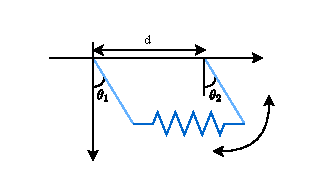
\includegraphics[width=0.6\textwidth]{res/svg/couple_pendulum_1.drawio}
    \caption{Coupled pendulums}
\end{figure}
The rest length of the spring is $d$. Since we have two particles, in principle we have at least $N=3\cdot2=6$ coordinates. Two coordinates can be neglected because the motion only occurs in the $xy$-plane.
The two ropes are a constraint on the position of the particles. In particular both constraints are holomonic and sclermonic:
\begin{equation}
    \begin{cases}
        x_1^2 + y_1^2 = l & \text{(first rope)}\\
        (x_2-d)^2 + y_2^2 = l & \text{(second rope)}
    \end{cases}
\end{equation}
We can write the transformation equations as follows:
\begin{equation}
    \begin{cases}
        x_1 = l\sin\theta_1\\
        y_1 = -l\cos\theta_1
    \end{cases}\;\;
    \begin{cases}
        x_2 = l\sin\theta_2+d\\
        y_2 = -l\cos\theta_2
    \end{cases}
\end{equation}
Since transformation equations do not depend on time the kinetic energy will be a quadratic function of the velocities:
\begin{equation}
    \begin{split}
        T &= \dfrac{1}{2}m(\underbrace{\dot{x}_1^2+\dot{y}_1^2}_{(l\dot{\theta}_1)^2}) + \dfrac{1}{2}m(\underbrace{\dot{x}_2^2+\dot{y}_2^2}_{(l\dot{\theta}_2)^2}) \\
        &= \dfrac{1}{2}ml^2(\dot{\theta}_1^2+\dot{\theta}_2^2)
    \end{split}
\end{equation}
We can express this in a matrix form as:
\begin{equation}
    \begin{split}
        T &= \dfrac{1}{2}(\dot{\theta}_1 \dot{\theta}_2)\hat{\Telegant}\begin{pmatrix}
            \dot{\theta}_1 \\\dot{\theta}_2
        \end{pmatrix} = \\
        &= \dfrac{1}{2}(\dot{\theta}_1 \dot{\theta}_2)ml^2\begin{pmatrix}
            1 & 0\\
            0 & 1
        \end{pmatrix}
        \begin{pmatrix}
            \dot{\theta}_1 \\\dot{\theta}_2
        \end{pmatrix} = \\
    \end{split}
\end{equation}
The potential is the sum of the gravitational potentials of the masses and of the elastic potential of the spring:
\begin{equation}
    \begin{split}
        V &= \underbrace{mgy_1 + mgy_2}_{-mgl(\cos\theta_1+\cos\theta_1)} + \dfrac{1}{2}k\left[\sqrt{(x_2-x_1)^2+(y_2-y_1)^2}-d\right]^2\\
        &= -mgl(\cos\theta_1+\cos\theta_1) +\\
        &+ \dfrac{1}{2}k\left[\sqrt{(l\sin\theta_2+d-l\sin\theta_1)^2+(l\cos\theta_1-l\cos\theta_2)^2}-d\right]^2\\
    \end{split}
\end{equation}
To find the minimum value of the potential we should theoretically evaluate the gradient and solve for $\grad V = \vec{0}$, but if we look at the configuration we can easily notice that the potential is minimum when the pendulums are in the vertical position and the spring is at rest as shown:
\\\textbf{IMMAGINE}\\
Thus we can expand the potential at $(0,0)$. Notice that the coordinates $\eta_1$ and $\eta_2$ in this case are equivalent to the ones we chose:
\begin{equation}
    \begin{split}
        V &\simeq V(0,0) +\dfrac{1}{2}\bigsum_{\alpha}\bigsum_{\beta} \dfrac{\partial^2 V}{\partial \theta_{\alpha} \partial \theta_{\beta}}\bigg|_{(0,0)}\theta_{\alpha}\theta_{\beta} = \\
        &= V(0,0) +\dfrac{1}{2}\brackets{\Velegant_{11}\theta_1^2 + \Velegant_{22}\theta_2^2 + 2\Velegant_{12}\theta_1\theta_2}
    \end{split}
\end{equation}
This can be expressed in matrix form:
\begin{equation}
    \begin{split}
        V &= \dfrac{1}{2}(\theta_1\;\theta_2)\hat{\Velegant}\begin{pmatrix}
            \theta_1 \\
            \theta_2
        \end{pmatrix}\\
        V &= \dfrac{1}{2}(\theta_1\;\theta_2)\begin{pmatrix}
            \Velegant_{11} & \Velegant_{12}\\
            \Velegant_{12} & \Velegant_{22}
        \end{pmatrix} \begin{pmatrix}
            \theta_1 \\
            \theta_2
        \end{pmatrix}
    \end{split}
\end{equation}
If we evaluate all the partial derivatives we get that the matrix $\hat{\Velegant}$ is:
\begin{equation}
    \hat{\Velegant} = \begin{pmatrix}
        mgl+kl^2 & -kl^2\\
        -kl^2 & mgl+kl^2
    \end{pmatrix}
\end{equation}
The Lagrangian finally looks like this:
\begin{equation}
    \lagr = \dfrac{1}{2}ml^2(\dot{\theta}_1^2+\dot{\theta}_2^2) - \dfrac{1}{2}\left[(mgl+kl^2)\theta_1^2 + 2(-kl^2)\theta_1\theta_2 + (mgl+kl^2)\theta_2^2 \right]
\end{equation}
And the \eleref\;are:
\begin{equation}
    \begin{cases}
        ml^2\ddot{\theta}_1 + (mgl + kl^2)\theta_1 - kl^2\theta_2 = 0\\
        ml^2\ddot{\theta}_2 + (mgl + kl^2)\theta_2 - kl^2\theta_1 = 0
    \end{cases}
\end{equation}
Dividing by $ml^2$ we get:
\begin{equation} \label{e:ode_system_double_pendulum}
    \begin{cases}
        \ddot{\theta}_1 + \brackets{\dfrac{g}{l} + \dfrac{k}{m}}\theta_1 - \dfrac{k}{m}\theta_2 = 0\\
        \ddot{\theta}_2 + \brackets{\dfrac{g}{l} + \dfrac{k}{m}}\theta_2 - \dfrac{k}{m}\theta_1 = 0
    \end{cases}
\end{equation}
And so we define a new matrix for the potential:
\begin{equation}
    \hat{\Velegant}' = \dfrac{\hat{\Velegant}}{ml^2}\begin{pmatrix}
        \dfrac{g}{l} + \dfrac{k}{m} & - \dfrac{k}{m}\\[10pt]
        - \dfrac{k}{m} & \dfrac{g}{l} + \dfrac{k}{m}
    \end{pmatrix}
\end{equation}
and for the kinetic energy:
\begin{equation}
    \hat{\Telegant}' = \dfrac{\hat{\Telegant}}{ml^2}\begin{pmatrix}
        1 & 0\\
        0 & 1
    \end{pmatrix}
\end{equation}
To find the eigenvalues we need to solve:
\begin{equation}
    \det(\hat{\Velegant}'-\lambda\mathbb{I}) = 0
\end{equation}
From which we get:
\begin{equation}
    \begin{split}
        \begin{vmatrix}
            \dfrac{g}{l} + \dfrac{k}{m} - \lambda & - \dfrac{k}{m}\\[10pt]
            - \dfrac{k}{m} & \dfrac{g}{l} + \dfrac{k}{m} - \lambda
        \end{vmatrix} &= 0\\
        \brackets{\dfrac{g}{l} + \dfrac{k}{m} - \lambda}^2 -\brackets{\dfrac{k}{m}}^2 & = 0\\
        \brackets{\dfrac{g}{l} + \cancel{\dfrac{k}{m}} - \lambda-\cancel{\dfrac{k}{m}}}\brackets{\dfrac{g}{l} + \dfrac{k}{m} - \lambda+\dfrac{k}{m}} &=0\\
        \brackets{\dfrac{g}{l} - \lambda}\brackets{\dfrac{g}{l} + 2\dfrac{k}{m} - \lambda} &=0
    \end{split}
\end{equation}
So we get the values for $\lambda_1$ and $\lambda_2$:
\begin{equation}
    \begin{split}
        \lambda_1 &= \dfrac{g}{l}\\
        \lambda_2 &= \dfrac{g}{l} + 2\dfrac{k}{m}
    \end{split}
\end{equation}
We want solutions like $\theta_i = a_i\efunction^{-i\omega t}$. Substituting this into \eqref{e:ode_system_double_pendulum} we get:
\begin{equation}
    \begin{cases}
        -\omega^2 a_1 \efunction^{-i\omega t} + \brackets{\dfrac{g}{l} + \dfrac{k}{m}} a_1 \efunction^{-i\omega t} - \dfrac{k}{m} a_2 \efunction^{-i\omega t} = 0\\[5pt]
        -\omega^2 a_2 \efunction^{-i\omega t} + \brackets{\dfrac{g}{l} + \dfrac{k}{m}} a_2 \efunction^{-i\omega t} - \dfrac{k}{m} a_1 \efunction^{-i\omega t} = 0
    \end{cases}
\end{equation}
Dividing by $\efunction^{-i\omega t}$ and remembering that $\omega^2 = \lambda$ we get:
\begin{equation}
    \begin{cases}
        \brackets{\dfrac{g}{l} + \dfrac{k}{m} - \lambda} a_1 - \dfrac{k}{m} a_2 = 0\\[5pt]
        -\dfrac{k}{m} a_1 + \brackets{\dfrac{g}{l} + \dfrac{k}{m} - \lambda} a_2 = 0
    \end{cases}
\end{equation}
Substituting $\lambda_1$ gives the eigenvector:
\begin{equation}
    \begin{cases}
        \brackets{\dfrac{g}{l} + \dfrac{k}{m} - \dfrac{g}{l}} a_1 - \dfrac{k}{m} a_2 = 0\\[5pt]
        -\dfrac{k}{m} a_1 + \brackets{\dfrac{g}{l} + \dfrac{k}{m} - \dfrac{g}{l}} a_2 = 0
    \end{cases}
\end{equation}
Simplifying, we get:
\begin{equation}
    \begin{cases}
        \dfrac{k}{m} a_1 - \dfrac{k}{m} a_2 = 0\\[5pt]
        -\dfrac{k}{m} a_1 + \dfrac{k}{m} a_2 = 0
    \end{cases}
\end{equation}
This implies:
\begin{equation}
    a_1 = a_2
\end{equation}
So the eigenvector corresponding to $\lambda_1$ is:
\begin{equation}
    \vec{a}^{\;(1)} = \begin{pmatrix}
        1\\
        1
    \end{pmatrix}
\end{equation}
Substituting $\lambda_2$ gives the eigenvector:
\begin{equation}
    \begin{cases}
        \brackets{\dfrac{g}{l} + \dfrac{k}{m} - \dfrac{g}{l} - 2\dfrac{k}{m}} a_1 - \dfrac{k}{m} a_2 = 0\\[5pt]
        -\dfrac{k}{m} a_1 + \brackets{\dfrac{g}{l} + \dfrac{k}{m} - \dfrac{g}{l} - 2\dfrac{k}{m}} a_2 = 0
    \end{cases}
\end{equation}
Simplifying, we get:
\begin{equation}
    \begin{cases}
        -\dfrac{k}{m} a_1 - \dfrac{k}{m} a_2 = 0\\[5pt]
        -\dfrac{k}{m} a_1 - \dfrac{k}{m} a_2 = 0
    \end{cases}
\end{equation}
This implies:
\begin{equation}
    a_1 = -a_2
\end{equation}
So the eigenvector corresponding to $\lambda_2$ is:
\begin{equation}
    \vec{a}^{\;(2)} = \begin{pmatrix}
        1\\
        -1
    \end{pmatrix}
\end{equation}
Any other vector which is a multiple of those vectors is an eigenvector. We want the normalized eigenvectors in order to construct an orthonormal basis. In this case the generalized normalization reduces to the regular one and we have:
\begin{equation}
    \vec{a}^{\;(1)} = \dfrac{1}{\sqrt{2}}\begin{pmatrix}
        1\\
        1
    \end{pmatrix}
\end{equation}
\begin{equation}
    \vec{a}^{\;(2)} = \dfrac{1}{\sqrt{2}}\begin{pmatrix}
        1\\
        -1
    \end{pmatrix}
\end{equation}
The solution can be written has:
\begin{equation}
    \vec{\theta} = u_1\vec{a}^{\;(1)}+u_2\vec{a}^{\;(2)}
\end{equation}
The orthonormality of the eigenvectors leads to:
\begin{equation}
    \begin{split}
        \vec{\theta} \cdot \vec{a}^{\;(1)} = u_1\\
        \vec{\theta} \cdot \vec{a}^{\;(2)} = u_2
    \end{split}
\end{equation}
We call $u_1$ and $u_2$ \textbf{normal modes} of the system.\\
If $u_1 =0$
\begin{equation}
    \vec{\theta} \cdot \vec{a}^{\;(1)} = (\theta_1\;\theta_2)\dfrac{1}{\sqrt{2}}\begin{pmatrix}
        1\\
        1
    \end{pmatrix} = \dfrac{\theta_1 + \theta_2}{\sqrt{2}} = 0
\end{equation}
Which implies:
\begin{equation}
    \theta_1 = -\theta_2
\end{equation}
Instead if we put $u_2=0$ we get:
\begin{equation}
    \vec{\theta} \cdot \vec{a}^{\;(2)} = (\theta_1\;\theta_2)\dfrac{1}{\sqrt{2}}\begin{pmatrix}
        1\\
        -1
    \end{pmatrix} = \dfrac{\theta_1 - \theta_2}{\sqrt{2}} = 0
\end{equation}
Which implies:
\begin{equation}
    \theta_1 = \theta_2
\end{equation}
This means that the first normal mode corresponds to a motion where the spring is never contracted and the pendulums move identically. The second normal mode corresponds to a motion of the pendulums in counterphase. Any other combination of the two modes is possible and we will have moments where the first mode is dominant and viceversa.
\section{The two body problem (WIP)}
